\chapter{Chapter2}\label{Chapter2}
\section{section21}\label{section21}
\subsection{subsection211 (\acs{LPE})}\label{subsection211}
\lipsum[1]

\subsection{subsection212}\label{subsection212}
\lipsum[1-2]


\begin{itemize}
\item
  the force due to the gravity can be expressed by Newton's
  3\textsuperscript{rd} law of motion
\item
  item 2
\item
  item 3
\end{itemize}

\lipsum[1-3]


%*******************************************************

\section{section22}\label{section22}
\subsection{subsection221}\label{subsection221}
\lipsum[1]


\begin{equation} 
A = \log_{10} (I_{0} \div I) = \log_{10} (100 \div T) = k \ast c \ast l
\label{eq:ch02eq1}
\end{equation}

\begin{equation} 
T = \exp (- \alpha \ast L)
\label{eq:ch02eq2}
\end{equation}

where:

\emph{I\textsubscript{0}} -- the intensity of the incident radiation,

\emph{I} -- the intensity of the transmitted radiation,

\emph{I}/\emph{I\textsubscript{0}} -- the transmittance (T) - often
presented in \%,

\emph{A} -- absorbance,

\emph{L} -- path length of the sample,

\emph{c} -- the concentration of the solution,

\emph{k} -- extinction coefficient (constant for the material, depends
on the wavelength of the radiation and nature of the molecule)

\emph{T} -- the transmission of the sample

\emph{$\alpha$\textsubscript{0}} -- the linear absorption coefficient
\\
\\

\lipsum[1]
\paragraph{paragraph:}
\lipsum[1]
%*******************************************************
\subsection{subsection222}\label{subsection222}
\lipsum[1]

\begin{figure}[!htb]
	\centering
	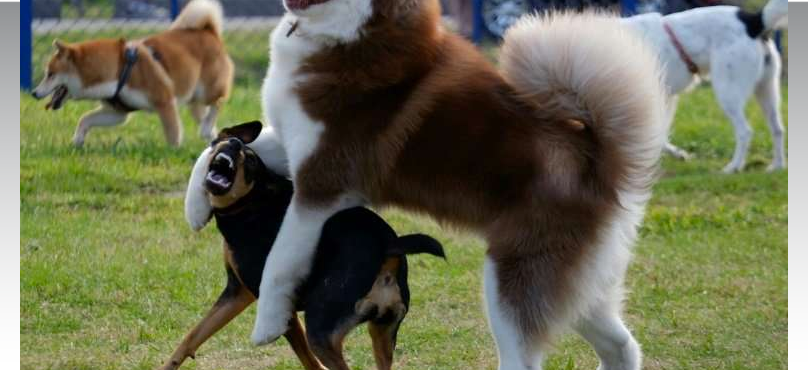
\includegraphics[width=.95\linewidth]{img/fig1.png} \quad
	\caption
	{
	Schematic describing the basic configurations
	}\label{fig:ch03f1}
\end{figure}

\paragraph{paragraph:}
\lipsum[1]
%*******************************************************

\subsection{subsection223}\label{subsection223}
\lipsum[1-3]
\paragraph{paragraph:}
\lipsum[1]
%*******************************************************

\subsection{subsection224}\label{subsection224}
\lipsum[1]
\paragraph{paragraph:}
\lipsum[1-3]
%*******************************************************

\subsubsection{subsection225}\label{subsection225}
\lipsum[1]
%*******************************************************

\subsection{subsection226}\label{subsection226}
\lipsum[1-2]
\paragraph{paragraph:}
\lipsum[1]
\paragraph{paragraph: }
\lipsum[1]
%*******************************************************